\documentclass[12pt,a4paper]{book}
\usepackage[utf8]{inputenc}
\usepackage[pdftex]{graphicx}
\usepackage[italian]{babel}
\usepackage{fixltx2e,bold-extra,geometry,
    amssymb,amsmath,mathtools, microtype,url,cite}
\usepackage[bookmarks=true, hidelinks, pdftitle={
SELEZIONE DI TOPOLOGIE D'ANTENNA MINIATURIZZATE SU MD},
pdfauthor={Alex Pacini}]{hyperref}
\usepackage{bold-extra}
\usepackage{listings}
\usepackage{xcolor}
\usepackage{caption}
\usepackage{minted}

\lstdefinelanguage{swift}
{
  morekeywords={
    func,if,then,else,for,in,while,do,switch,case,default,where,break,continue,fallthrough,return,
    typealias,struct,class,enum,protocol,var,func,let,get,set,willSet,didSet,inout,init,deinit,extension,
    subscript,prefix,operator,infix,postfix,precedence,associativity,left,right,none,convenience,dynamic,
    final,lazy,mutating,nonmutating,optional,override,required,static,unowned,safe,weak,internal,
    private,public,is,as,self,unsafe,dynamicType,true,false,nil,Type,Protocol,
    UIViewController,UINavigationController,Bool
  },
  morecomment=[l]{//}, % l is for line comment
  morecomment=[s]{/*}{*/}, % s is for start and end delimiter
  morestring=[b]" % defines that strings are enclosed in double quotes
}

\definecolor{keyword}{HTML}{BA2CA3}
\definecolor{string}{HTML}{D12F1B}
\definecolor{comment}{HTML}{008400}

\lstset{
  language=swift,
  basicstyle=\ttfamily,
  showstringspaces=false, % lets spaces in strings appear as real spaces
  columns=fixed,
  keepspaces=true,
  keywordstyle=\color{keyword},
  stringstyle=\color{string},
  commentstyle=\color{comment},
}


\pagestyle{headings}
\graphicspath{{images/}}

%%%%%%%%%%%%%%%%% New Commands %%%%%%%%%%%%%%%%%%%%%%%%%%%%%%%%%%%%%%%%%%%%%%%%%
%
\newcommand{\intentblankpage}{
%     Leaves a blank page
    \newpage
    \null
    \vfill
    \thispagestyle{empty}
%     \begin{center}
% %         \textit{This page intentionally left blank.}
%         % \textit{Questa pagina \`e lasciata intenzionalmente bianca.}
%     \end{center}
    \newpage
}
% 
% Writes intentionally blank page when there is a \newpage on the left page of
% a book.
\makeatletter
    \def\cleardoublepage{\clearpage%
        \if@twoside
            \ifodd\c@page\else
                \vspace*{\fill}
                \hfill
                \begin{center}
%                     \textit{This page intentionally left blank.}
                    % \textit{Questa pagina \`e lasciata intenzionalmente bianca.}
                \end{center}
                \thispagestyle{empty}
                \newpage
                \if@twocolumn\hbox{}\newpage\fi
            \fi
        \fi
    }
\makeatother
%
% Length to set margins for 65 chars
\newlength{\sixtyfivecharwidth}
\settowidth{\sixtyfivecharwidth}{
    \normalfont abcdefghijklmnopqrstuvwxyzabcdefghijklmnopqrstuvwxyz1234567890123}
% 
%Integral with the limit below(mathrlap)
% \newcommand{\intlimr}[1]{\ensuremath{\int \limits_{\mathrlap{#1}}}}
% 
% This redefine could cause big issues! See: 
% http://tex.stackexchange.com/questions/248421/use-mathclap-as-default-in-limits-of-integration
% \let\oldlimits\limits
% \def\limits_#1{\oldlimits_{\mathclap{#1}}}
\def\mclimits_#1{\limits_{\mathclap{#1}}}
%%%%%%%%%%%%%%%% End New Commands %%%%%%%%%%%%

\begin{document}
    \pagenumbering{Roman}
    % \newgeometry{margin=26mm} % allarga la pagina anche in altezza
\newgeometry{lmargin=21mm,rmargin=21mm}
\begin{titlepage}
\begin{center}
    
\includegraphics[scale=0.35]{logo.png}\\
    \vspace{8mm}
    {\huge{\textsc{\textmd{Università degli studi di Udine}}}}\\
    \vspace{10mm}
    {\large{\textbf{ Dipartimento di Scienze Matematiche, Informatiche e Fisiche}}}\\
    \vspace{0.5cm}
    {\large{\textbf{ Corso di laurea in Tecnologie Web Multimediali}}}
\end{center}
\vspace{10mm}
\begin{center}
    {\LARGE\textbf{\textsc{Progettazione e sviluppo di}}}\\
    \vspace{6mm}
    {\LARGE\textbf{\textsc{un'applicazione per la}}}\\
    \vspace{6mm}
    {\LARGE\textbf{\textsc{fidelizzazione e il rewarding}}}\\
    \vspace{6mm}
    {\LARGE\textsc{\textbf{degli utenti}}}\\
    \vspace{10mm}
\end{center}
\vfill
\par
\noindent
% \begin{minipage}[t]{0.47\textwidth}
%     \vspace{10mm}
%     \thinspace{\large{\sc Relatore}\\
%     \vspace{2mm}
%     {\bf Prof. STEFANO BURIGAT}}
% \end{minipage}
% \hfill
% \noindent
% \begin{minipage}[t]{0.47\textwidth}\raggedleft
%     \vspace{10mm}
%     {\large{\sc Laureando}\\
%     \vspace{2mm}
%     {\bf RICCARDO CARANFIL}}
% \end{minipage}

\begin{minipage}[t]{0.47\textwidth}
    \vspace{13mm}
    \large{\sc Relatore}\\
\end{minipage}
\hfill
\noindent
\begin{minipage}[t]{0.47\textwidth}\raggedleft
    \vspace{13mm}
    \large{\sc Laureando}\\
\end{minipage}

\begin{minipage}[t]{0.47\textwidth}
    \large\bf{Prof. STEFANO BURIGAT}
\end{minipage}
\hfill
\begin{minipage}[t]{0.47\textwidth}\raggedleft
    \large\bf{RICCARDO CARANFIL}
\end{minipage}

\vspace{18mm}
\begin{center}
    % {\large{\sc I Appello - I Sessione}
    {\rule[0.2cm]{5cm}{0.3mm}\\
    %inserire il numero della sessione in cui ci si laurea
    \large{\sc{Anno Accademico 2018/2019}}}
    %inserire l'anno accademico a cui si è iscritti
\end{center}
\end{titlepage}
\restoregeometry

    \intentblankpage
    
    \newgeometry{text={\sixtyfivecharwidth,35\baselineskip}}
    \vspace*{50mm}
    %\begin{flushright}
    %     {\Large{\bf Keywords:}\\ \vspace{5mm}
    %         Magneto-Dielettrico\\ \vspace{2mm}
    %         Correnti Superficiali\\ \vspace{2mm}
    %         Topologie di Antenne\\ \vspace{2mm}
    %         Far-Field\\
    %     }
    % \end{flushright}
        
    \vspace*{50mm}
    \begin{flushright}
        \textit{\large Ringrazio la mia famiglia e tutti i miei amici per avermi accompagnato lungo questo percorso}
    \end{flushright}
    
    \newpage
    
    % \vspace*{30mm}
    % \begin{flushright}
    %     \textit{\large Citazione 
    %         \\ \vspace{5mm}  - Tizio Caio -}
    % \end{flushright}
    
    % \vfill
    
    % \noindent \hspace{20mm} \textit{\large{Ringraziamenti:}} \vspace{5mm}\\
    % Da scrivere
    
    % \newpage
    \tableofcontents
    
    \chapter*{Introduzione}
    \pagenumbering{arabic}
    \addcontentsline{toc}{chapter}{Introduzione}  
    \normalsize
L’obiettivo principale del tirocinio presso \textbf{Urbana Smart Solutions srl}\cite{urbanasmartsolutions}
è stata la creazione di un'applicazione
iOS denominata \textbf{QIX} atta alla fidelizzazione e al rewarding di un target di utenti specifico. 
Il principali target di clienti a cui mira l'applicazione sono delle FMCG\footnote{Fast Moving Consumer
Goods}, ossia delle compagnie che vendono beni di consumo a basso
costo e molto velocemente.

Tali compagnie attraverso i loro prodotti possono creare diverse
tipologie di eventi e gli utenti dell’applicazione possono accedervi
e vincere dei punti denominati \textbf{QIX coins} con cui comprare o avere degli
sconti sui beni venduti.

% Esistono diverse modalità in cui un utente può accadere a tali eventi:
% \begin{itemize}
%     \item Usando la funzione “shake” dello smartphone in determinati contesti;
%     \item Usando specifiche funzioni come la G'morning Challenge o la ruota della fortuna;
% \end{itemize}

L’elemento cardine dell’app è il \textbf{QIX Shake} ossia l’attivazione di un particolare servizio
che dipende dal contesto attuale dell'utente e il tipo di offerta che viene selezionata.
Tale servizio dà agli la possibilità di vincere dei QIX coins agitando lo smartphone.
I principali servizi di shake dell'applicazione sono:

\begin{enumerate}
    \item\textbf{TV Shake}: agitando lo smartphone inizierà un'analisi dei dati del microfono
    allo scopo di trovare un particale \textbf{watermark} inserito in campagnie publicitarie televisive;
    \item\textbf{Read Shake}: all'utente viene proposta la lettura di contenuti o questionari in cambio di QIX coins;
    \item\textbf{Video Shake}: a seguito della visualizzazione di uno video l'utente viene premiato con dei punti;
    \item\textbf{Scan shake}: dopo aver scannerizzato il barcode di un prodotto (Es. al supermercato) all'utente verrano assegnati dei punti;
    \item\textbf{Receipt Shake}: dopo aver scannerizzato uno scontrino di acquisto di prodotti partner delle FCMG;
    \item\textbf{Stadium Shake}: inierà anche in questo caso l'analisi del suono esterno per la ricerca di eventuali watermark
    generati in un'audio durante delle partite allo stadio;
\end{enumerate}


    
    \chapter{Progettazione iniziale}
    \label{CH:1}
    
Il mio compito nello sviluppo dell'applicazione è stato quello 
di creare un \textbf{prototipo} iniziale avendo a disposizione un mock up creato con
proto.io\cite{protoio} e una serie di requisiti essenziali.

\subsection{Mock up iniziale}

Il prototipo iniziale dell'applicazione prevede una
bottom TabBar con cinque elementi ognuno dei quali
descrivere le seguenti funzionalità:

\begin{enumerate}
    \item \textbf{Storico delle offerte}: è stato implementato attraverso un pattern Overview and Details
    e consiste in una lista in cui l'utente può visualizzare i dettagli cliccando sull'offerta desiderata.
    \item \textbf{Tutte le offerte}: la vista è strutturata con un filtro per categoria nella parte superiore,
    con cui l'utente può controllare tutte le offerte disponibili. Tutte le offerte offrono una tipologia di QIX Shake diversa tra quelle elencate nell'introduzione.
    \item \textbf{Sezione Scan}: la sezione scan sarà utilizzata per lo scanning di QR Code o di scontrini d'acquisto da parte dell'utente,
    così che possa guadagnare dei QIX Coins.
    \item \textbf{Gift Cards}: in questa sezione l'utente potrà comprare delle gift cards digitali o materiali usando i suoi QIX Coins.
    \item \textbf{Sezione Me}: in questa view vengono mostrati tutti i dati riguardanti l'utente, il supporto tecnico
    e la funzione per invitare gli amici.
\end{enumerate}

Oltre alle viste principali ho creato anche un onboarding in cui l'utente può decidere se effetture la registrazione
attraverso il proprio numero di telefono o entrare direttamente nell'app come utente Guest, un esempio della registrazione è
visibile nell figura~\ref{fig:screenshots} (d).

\begin{figure}
    \hfill
    \subfigure[Storico offerte]{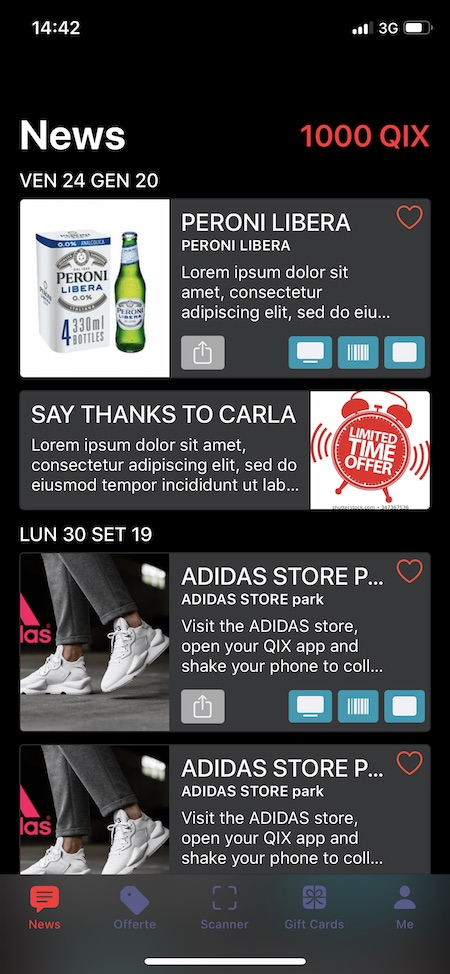
\includegraphics[width=3.2cm]{screen_1}}
    \hfill
    \subfigure[Tutte le offerte]{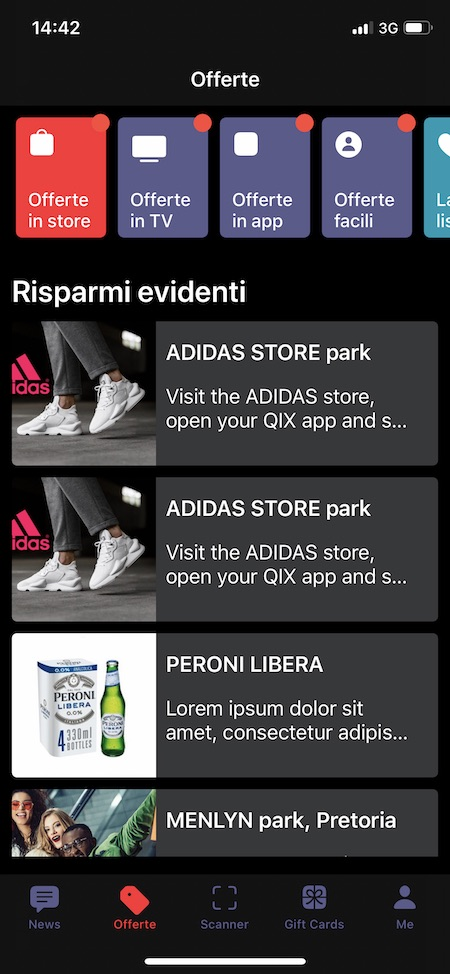
\includegraphics[width=3.2cm]{screen_2}}
    \hfill
    \subfigure[Sezione Me]{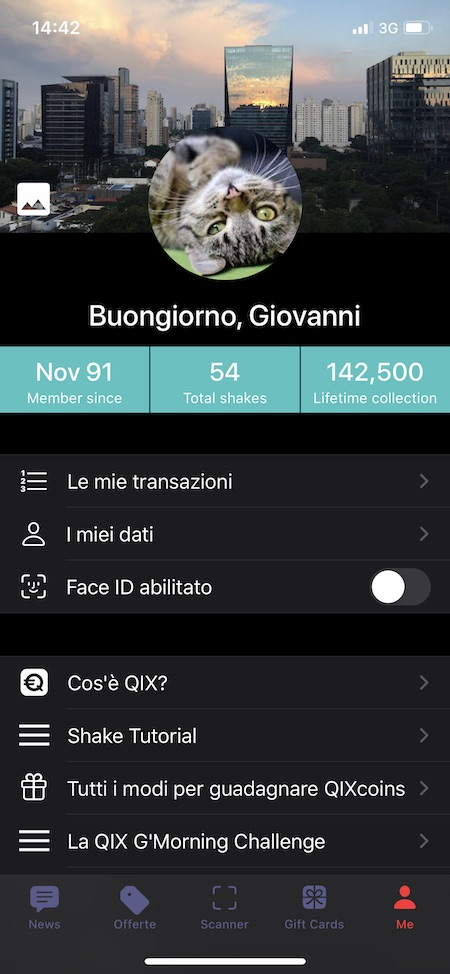
\includegraphics[width=3.2cm]{screen_3}}
    \hfill
    \subfigure[Registrazione]{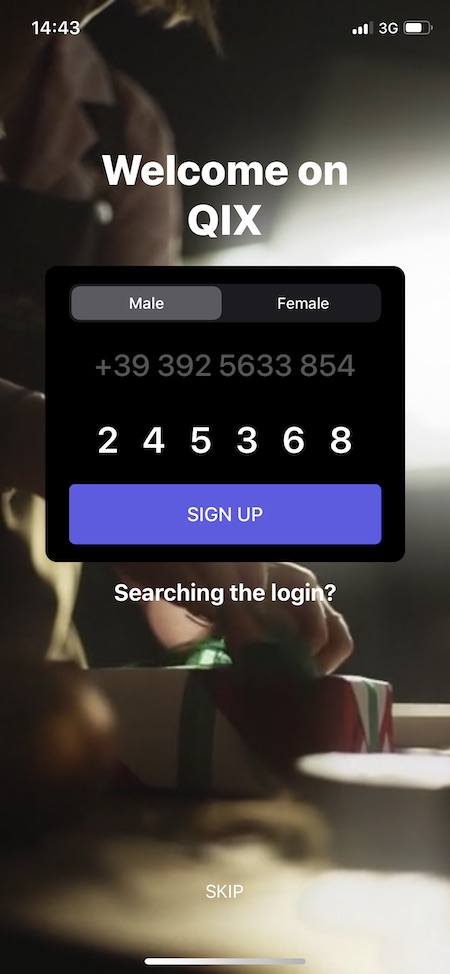
\includegraphics[width=3.2cm]{screen_4}}
    \hfill
    \caption{Screenshots prototipo iniziale}\label{fig:screenshots}
\end{figure}

In particolare, come spiegherò nella sezione~\ref{sec:coordinator}, è stato utilizzato il Coordinator Pattern
per la gestione delle viste ed ogni view visibile in figura~\ref{fig:screenshots} è un esempio di UIViewController
figlio di un CoordinatorNavigable.

\subsection{Requisiti}
La base di partenza di QIX sono state delle funzionalità essenziali e 
sostanzialmente molto difficili da inserire in una versione dell'app già avanzata.
È stato quindi deciso di creare un prototipo di partenza avente i seguenti requisiti:

\begin{itemize}
    \item {
        \textbf{Navigazione dinamica}: L'applicazione deve gestire dei cambiamenti di contesto
        dinamici: dev'essere possibile mostrare all'utente contenuti dinamici indipendentemente
        dal contesto in cui si trova. 
    }
    \item {
        \textbf{QIX Shake}: L'utente deve poter agitare lo smartphone in qualsiasi
        sezione dell'applicazione e il risultato deve essere basato sul contesto attuale o su delle direttive dettate
        da delle Rest API.
    } 
    \item {
        \textbf{Animazioni interattive}: L'intera applicazione dev'essere progettata in modo tale da presentare all'utente
        delle \textbf{animazioni interattive} in stile CardView\cite{cardview} disponibili in 
        qualunque sezione o vista in cui si trovi l'utente e definite dal contesto attuale.

        Le animazioni in questione devono essere progettate in pagine, ciascuna delle quali può contenere 
        più CardView. L'utente vedrà in un determinato momento una e soltanto una pagina.

        Ogni CardView deve essere trascinabile dall'utente e deve interagire con le altre CardView della pagine. 
        Quando l'utente usa una forza di trascinamento superiore a un valore di soglia tutte le viste devono
        cadere per gravità.
        
        Tale gravità finirà con la fine dell'animazione o l'apparizione di una nuova pagina se presente.
    }
    \item {
        \textbf{Autenticazione}: L'applicazione deve supportare tre diversi stati o modalità di autenticazione:
        \begin{enumerate}
            \item\textbf{Trial Mode}: l'utente è anonimo, esiste solo un id per tenere traccia dei suoi QIX coins.
            \item\textbf{Signed Mode}: l'utente ha inserito il numero di telefono e il suo genitore.
            \item \textbf{Pro Mode}: l'utente aggiunge dei dati su se stesso o collega il suo account a dei social media come Facebook, Google o Instagram.
        \end{enumerate}
        Si nota facilmente che non esiste una stato in cui l'utente non è registrato: questo perchè
        per tenere traccia dei suoi QIX coins e di altri dati utili è necessario avere una riferimento all'utente.
    }
    \item {
        \textbf{DeepLinks}: L'applicazione deve poter essere avviata dinamicamente
        attraverso dei \textbf{Deep Links}\cite{deeplinks}.
        E deve essere in grado di gestirli in base al contesto dell'utente.
    }
\end{itemize}
    
    \chapter{Componenti base di iOS }
    \label{CH:2}
    
% Analizzando il requisito mi sono posto diverse domande: \\ \\
% \noindent{
%     \large\textit{Cosa significa dinamicamente?}
%     \normalsize{Il nostro obiettivo in questo caso è mostrare all'utente \textbf{contenuti diversi}
%     indipendentemente dal constesto e quindi dalla vista in cui si trova}\\ \\
%     \large\textit{Quale contesto?}
%     \normalsize{Con contesto dell'utente si intende lo stato attuale dell'applicazione,
%     quindi l'intero stack di navigazione se presente;
%     } \\ \\
% }

Prima di entrare nel merito delle soluzioni e problemi affrontati, elenco brevemente gli strumenti
base di iOS che mi sono stati utile nella progettazione e implementazione finale.

\section{Navigazione standard}

Un'applicazione iOS è un insieme di \textbf{UIViewController}\cite{viewcontroller} diversi che 
regolano ogni aspetto della lora vista;

% Qualsiasi applicazione ha infatti un rootViewController, ossia un ViewController di partenza

Ogni applicazione può avere degli \textbf{UINavigationController}\cite{navigationcontroller},
ossia dei contenitori di \textbf{UIViewController} che vengono
utilizzati per mantenere lo stack di navigazione e gestire la transizioni tra due UIViewController.

Nella figura~\ref{fig:1} si nota facilmente come un NavigationController gestisce un'array di ViewController e una sola 
navigation bar. \\
% In iOS sono infatti innate molte animazioni di navigazione che è utile sfruttare, piuttosto di creare 
% componenti custom poi difficili da rendere interattivi.\\

\begin{minipage}{\linewidth}
    \centering
    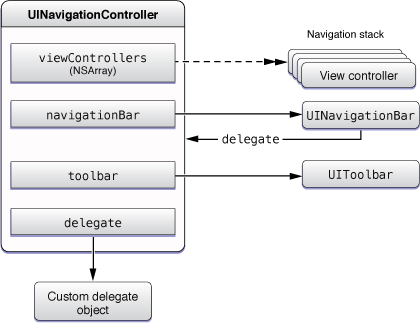
\includegraphics[width=5cm]{navigation}
    \captionof{figure}{Navigation controller scheme}
    \label{fig:1}
\end{minipage}

\subsection{Tipologie di navigazione}\label{sec:navigation}

Esistono tre tipologie base di navigazione:

\begin{enumerate}
    \item{\textbf{Push}: un UIViewController figlio di un NavigationController può rendere
    visibile un altro ViewController attraverso la funzione "pushViewController" di un Navigation controller\par
    \begin{minipage}{\linewidth}
        \centering
        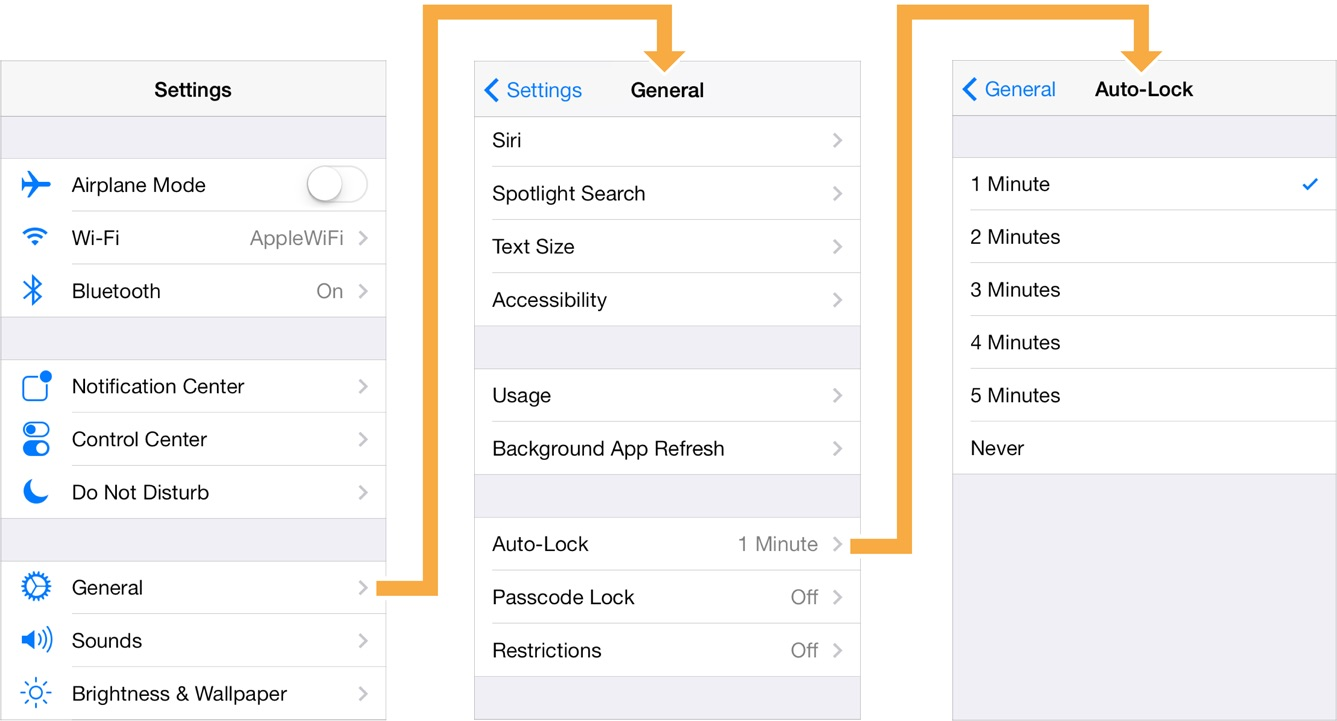
\includegraphics[width=10cm]{push}
        \captionof{figure}{Presantazione di un ViewController tramite push}
        \label{fig:2}
    \end{minipage}
    }
    \item{ \textbf{Modal}: un ViewController può presentare un altro ViewController senza necessariamente avere un 
        Navigation Controller, l'animazione standard è dal basso verso l'alto come in figura~\ref{fig:3}\par
        \begin{minipage}{\linewidth}
            \centering
            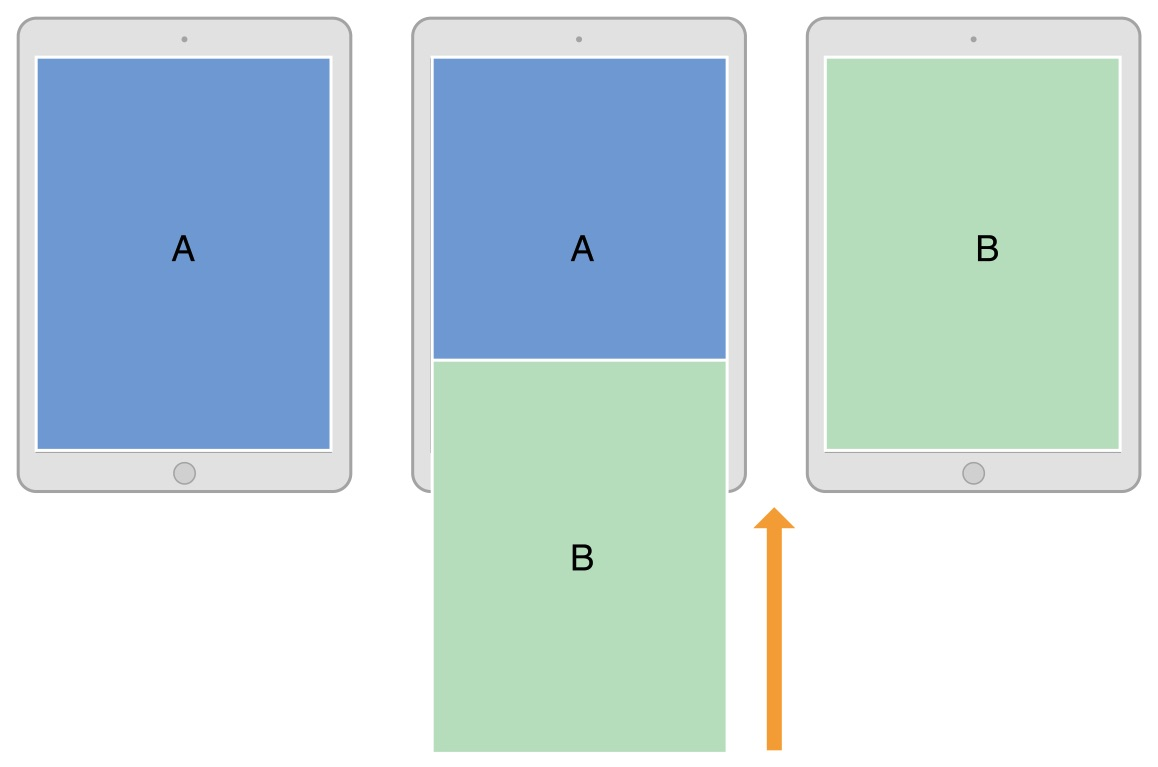
\includegraphics[width=10cm]{modal}
            \captionof{figure}{
                Presantazione di un ViewController tramite modal
            }
            \label{fig:3}
        \end{minipage}
    }
    \item{\textbf{Segue}: Una segue non è altro che un link tra due view controller attraverso un'interfaccia
        grafica. In base alla tipologia cambia il tipo di navigazione (Modal o Push)
    }
\end{enumerate}

% Avendo definito i principali metodi di navigatione tra ViewController torniamo al problema iniziale:
% \textit{Come possiamo rendere dinamica la navigazione?}

% A seguito di uno studio approfondito di varie tecniche di navigazione iOS ho scelto di utilizzare il
% \textbf{Coordinator Pattern}\cite{coordinatorpattern}.

% \section{Il Coordinator Pattern}

% Generalmente in iOS l'intera logica di un ViewController viene scritta nel ViewController stesso, creando spesso
% file di grosse dimensioni e disordine generale. Il Coordinator Pattern è nato proprio per rendere 
% le applicazioni più scalabili e leggere. 

% Ogni ViewController infatti delega tutte le decisioni al suo Coordinator che in base a determinate logiche deciderà
% i passi successivi.

% Ogni Coordinator può controllare un ViewController o più Coordinator, questo rende le viste
% indipendenti tra di loro e rende ogni ViewControler totalmente invisibile agli altri.\\

% \begin{minipage}{\linewidth}
%     \centering
%     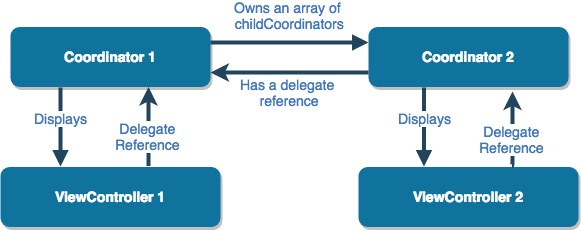
\includegraphics[width=10cm]{coordinator}
%     \captionof{figure}{
%         Il Coordinator Pattern
%     }
%     \label{fig:4}
% \end{minipage}\\ \\

% La resposibilità dei coordinator è infatti la navigazione, come un navigation controller gestisce i sui View Controller, un coordinator gestisce
% i suoi figli e questo rende ogni vista o flow di navigazione totalmente indipendente dal resto dell'applicazione.

% Per navigare tra i view controller vengono generalmente usate le tipologie di navigazione
% descritte nella sezione~\ref{sec:navigation}, tranne le segue, che essendo definete da vista grafica renderebbero
% la navigazine statica e fissata su determinati ViewController. \\

% Di seguito in figura~\ref{fig:5} presento uno schema dell'utilizzo di due coordinator
% per la gestione di una lista di prodotti e il carrello. \\

% \begin{minipage}{\linewidth}
%     \centering
%     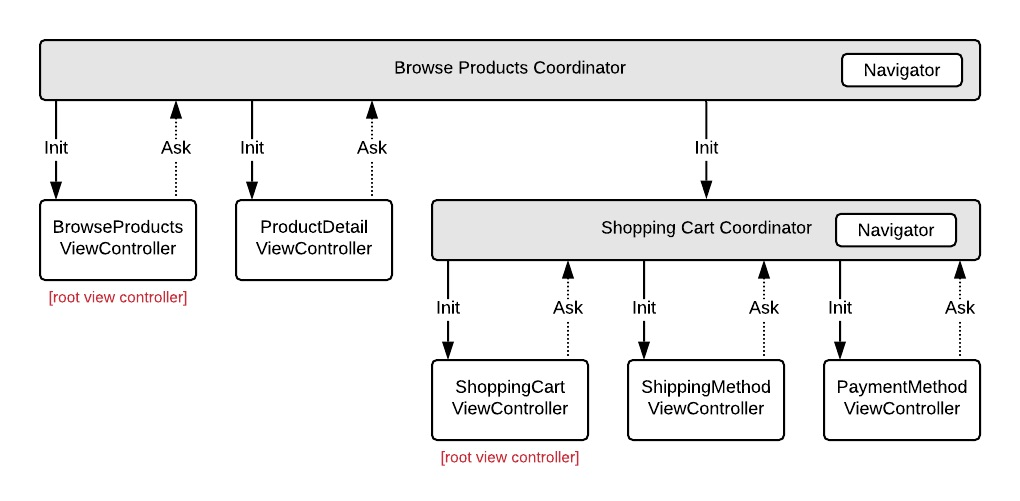
\includegraphics[width=10cm]{coordinator-example}
%     \captionof{figure}{
%        Esempio di coordinator pattern
%     }
%     \label{fig:5}
% \end{minipage}\\ \\

% Come si evince dall'immagine è presente in entrambi i coordinator è presente un oggetto
% \textbf{navigator} che sarà in gestore di un UINavigationController
\section{UIKit Dynamics}

Per la progettazione iniziale delle animazioni è stato fatto un attento studio a metodologie e frameworks
atti a creare animazioni interattive fluide.

Alla fine è stato deciso di utilizzare un pacchetto
nativo di iOS incluso nello UIKit\cite{uikit}, chiamato UIKit Dynamics\cite{uidynamics}: questo framework,
con una serie di API, offre delle funzioni di animazione base che 
donano alle viste i comportamenti fisici del mondo reale.

Il framework si basa su degli oggetti \textbf{UIDynamicAnimator} in cui ogni animator è responsabile delle
animazioni che avengono sulla sua \textbf{referenceView} e si inizializza 
attraverso la seguente funzione:

\begin{minted}{swift}
    UIDynamicAnimator.init(referenceView view: UIView)
\end{minted}

% una volta inizializzato attraverso la funzione addBehavior sarà posibile assegnargli
% dei comportamenti fisici predefiniti.

\subsection{Comportamenti base}

Ogni animator attraverso il metodo addBehavior puà assegnare a determinate
viste comportamenti fisici elencati sei seguito: 

\begin{itemize}
    % \item\textbf{UIDynamicBehavior}: il comportamento base da cui ereditano tutti gli altri;
    \item\textbf{UIAttachmentBehavior}: crea una relazione o legame tra due DynamicItem o tra un DynamicItem e un punto di ancoraggio;
    \item\textbf{UICollisionBehavior}: un oggetto che conferisce a un array di DynamicItems la possibilità di impegnarsi in collisioni tra loro e con i limiti specificati del comportamento
    \item\textbf{UIFieldBehavior}: un oggetto che conferisce delle proprietà magnetiche, elettriche a un DynamicItem;
    \item\textbf{UIGravityBehavior}: aggiunge all'oggeto un forza di gravità;
    \item\textbf{UIPushBehavior}: Aggiunge all'oggetto una forza continua o istantanea in una direzione specifica;
    \item\textbf{UISnapBehavior}: Un comportamento simile a una molla il cui movimento iniziale viene smorzato nel tempo in modo che l'oggetto si stabilizzi in un punto specifico.
\end{itemize}

Di seguito un esempio di implementazione degli strumenti UIDynamics in QIX

\begin{minipage}{\linewidth}
    \centering
    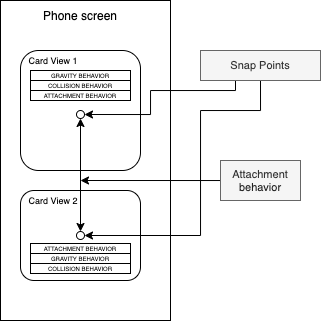
\includegraphics[width=10cm]{animation}
    \captionof{figure}{
       Schema dell'implementazione di UIDynamics
    }
    \label{fig:6}
\end{minipage}\\

    \chapter{Navigazione dinamica}
    \label{CH:3}
    

Avendo definito i principali metodi di navigatione tra ViewController al capitolo~\ref{CH:2} torniamo al problema iniziale:
\textit{Come possiamo rendere dinamica la navigazione?}

A seguito di uno studio approfondito di varie tecniche di navigazione iOS ho scelto di utilizzare il
\textbf{Coordinator Pattern}\cite{coordinatorpattern}.

\section{Il Coordinator Pattern}

Generalmente in iOS l'intera logica di un ViewController viene scritta nel controller stesso, creando spesso
file di grosse dimensioni e disordine generale. Il Coordinator Pattern è nato proprio per rendere 
le applicazioni più scalabili e leggere. 

Ogni ViewController infatti delega tutte le decisioni al suo Coordinator usando il Delegation Pattern (vedere sezione~\ref{delegation}) che in base alle logiche
della vista in questione deciderà i passi successivi.

Ogni Coordinator può controllare un ViewController o più Coordinator, questo rende le viste
indipendenti tra di loro e rende ogni ViewControler totalmente invisibile agli altri.\\

\begin{minipage}{\linewidth}
    \centering
    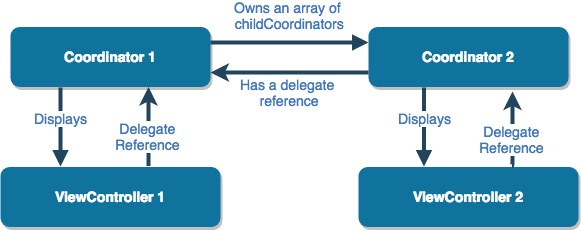
\includegraphics[width=10cm]{coordinator}
    \captionof{figure}{
        Il Coordinator Pattern
    }
    \label{fig:4}
\end{minipage}\\ \\

La resposibilità dei coordinator è infatti la navigazione, come un navigation controller gestisce i sui View Controller, un coordinator gestisce
i suoi figli e questo rende ogni vista o flow di navigazione totalmente indipendente dal resto dell'applicazione.

Per navigare tra i view controller vengono generalmente usate le tipologie di navigazione
descritte nella sezione~\ref{sec:navigation}, tranne le segue, che essendo definete da vista grafica renderebbero
la navigazine statica e fissata su determinati ViewController. \\

Di seguito in figura~\ref{fig:5} presento uno schema dell'utilizzo di due coordinator
per la gestione di una lista di prodotti e il carrello. \\

\begin{minipage}{\linewidth}
    \centering
    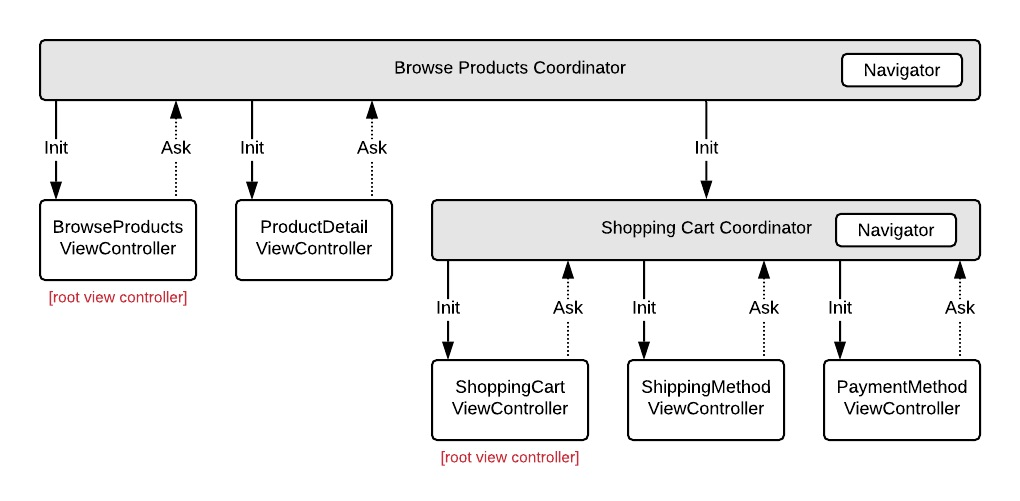
\includegraphics[width=10cm]{coordinator-example}
    \captionof{figure}{
       Esempio di coordinator pattern
    }
    \label{fig:5}
\end{minipage}\\ \\

Come si evince dalla figura~\ref{fig:5} è presente in entrambi i coordinator un oggetto
\textbf{navigator} che sarà il proxy di un generico UINavigationController

\section{Implementazione}

Ogni coordinator ha degli elementi fissi che sono:

\begin{itemize}
    \item Una funzione di partenza denominata \textbf{start};
    \item Un array di coordinator figli;
\end{itemize}

Per questo ho iniziato implementando dei protocolli:
\subsection{Protocolli base}

Il primo protollo implememtato è quello che defisce un qualunque coordinator
e ne tiene in memoria i figli in modo che non vengano
dealloccati automaticamente dal sistema operativo.

\begin{minted}{swift}
protocol Coordinator: class {

    var childCoordinators: [Coordinator] { get set }
    
    /** Utilizzato task di inizializzazione */
    func start()
    
}

extension Coordinator {
    
    // Aggiunge un figlio al coordinator padre
    func add(childCoordinator: Coordinator) {
        childCoordinators.append(childCoordinator)
    }
    
    // Rimuove un Coordinator figlio dal parent
    func remove(childCoordinator: Coordinator) {
        childCoordinators = childCoordinators.filter {
            $0 !== childCoordinator 
        }
    }
}
\end{minted}

Successivamente è stato implementato un BaseCoordinatorPresentable, che estende Coordinator
e aggiunge delle funzionalità di presentazione modale.

\begin{minted}{swift}
protocol BaseCoordinatorPresentable: Coordinator {

    // Il view controller principale del coordinator
    var _rootViewController: UIViewController { get }
}

// MARK: - Presentation Methods

extension BaseCoordinatorPresentable {
    
    /**
     Inizia un coordinator figlio e presenta
     il suo rootViewController modalmente

     - Parametri:
        - childCoordinator: Il coordinator da presentare
        - animated: Specifica se con o senza animazione modale
     */
    
    func presentCoordinator(_ childCoordinator: BaseCoordinatorPresentable,
        animated: Bool) {

        add(childCoordinator: childCoordinator)
        childCoordinator.start()
        _rootViewController.present(childCoordinator._rootViewController, animated: animated)
    }
    
    /**
     Inizia un viewController senza coordinator e
     lo presenta modalmente
     
     - Parametri:
        - controller: Il controller da presentare
        - animated: Specifica se con o senza animazione modale
     */
    
    func present(_ controller: UIViewController, animated: Bool) {
        _rootViewController.present(controller, animated: animated)
    }
    
    /**
     Interrompe la presentazione di un child Coordinator
     eliminandolo anche dall'array in memoria

     - Parameters:
        - childCoordinator: Il coordinator da chiudere e rilasciare
        - animated: Specifica se con o senza animazione modale
        - completion: closure che viene eseguita alla vine del dismiss
     */
    
    func dismissCoordinator(_ childCoordinator: BaseCoordinatorPresentable,
        animated: Bool, completion: (() -> Void)? = nil) {

        childCoordinator._rootViewController.dismiss(animated: animated,
            completion: completion)
        self.remove(childCoordinator: childCoordinator)
    }

}
\end{minted}

\subsection{Coordinator modale}

Il BaseCoordinatorPresentable è stato definito per evitare errori di \textbf{associetedtype},
infatti questo protocollo non deve mai essere implemetato direttamente, ma soltanto con il protocollo sucessivo

\begin{minted}{swift}
protocol CoordinatorPresentable: BaseCoordinatorPresentable {

    /**
        Questo protocolo utilizza la tipizzazione per
        permettere di ottenere Coordinator con view
        controller tipizzati.
     */
    associatedtype ViewController: UIViewController

    // Il rootViewController del coordinator
    var rootViewController: ViewController { get }

}

extension CoordinatorPresentable {

    // Ritorna rootViewController
    var _rootViewController: UIViewController {
        return rootViewController
    }
}
\end{minted}

\section{Aggiunta del Navigator}

Successivamente ho creato un protocollo \textbf{CoordinatorNavigable} che estende 
il coordinator visto in precedenza e ne aggiunge un oggetto navigator:

\begin{minted}{swift}
protocol CoordinatorNavigable: CoordinatorPresentable {
    
    /** Responsabile dello stack di navigazione  */
    var navigator: Navigator { get }
}

extension CoordinatorNavigable {
    
    /**
     Aggiunge il rootViewController allo stack di navigazione
    */
    func pushCoordinator(_ childCoordinator: BaseCoordinatorPresentable,
            animated: Bool) {
        add(childCoordinator: childCoordinator)
        childCoordinator.start()
        navigator.push(childCoordinator._rootViewController,
                animated: animated,
                onPoppedCompletion: { [weak self] in
                    self?.remove(childCoordinator: childCoordinator)
        })
    }
}

final class Navigator: NSObject {

    private let navigationController: UINavigationController
    private var completions: [UIViewController: () -> Void]
    
    init(navigationController: UINavigationController = UINavigationController()) {
        self.navigationController = navigationController
        self.completions = [:]
        
        super.init()
        
        self.navigationController.delegate = self
    }
}
\end{minted}

Come si può osservare dall'esempio riportato precedentemente il \textbf{Navigator}
ha lo scopo di tenere in memoria un UINavigationController che sarà il vero 
responsabile della navigazione.

\subsection{Utilizzo del pattern in QIX}

In QIX è stato creato un Coordinator principale deniminato AppCoordinator che gestisce
tutto lo startup dell'applicazione: decide quale vista mostrare e controlla se ci sono dei dynamic links in arrivo.
Tutta la struttura attuale dell'applicazione è invece costruita sul MainTabBarCoordinator, ossia il responsabile
della TabBar e di tutti i coordinator suoi figli.\\

\begin{minipage}{\linewidth}
    \centering
    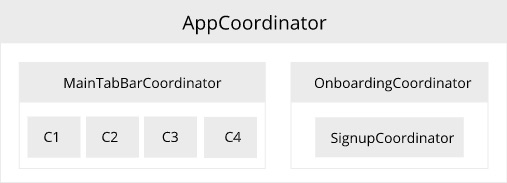
\includegraphics[width=10cm]{qix_coord}
    \captionof{figure}{
       Il Coordinator pattern in QIX
    }
    \label{fig:6}
\end{minipage}\\ \\

Tale struttura è stata creata per permettere modifiche future semplici e scalabili.
Esiste solo un vincolo ossia un rootCoordinator, ossia colui che gestirà il primissimo viewController dell'applicazione, in questo caso è MainTabbarCoordinator ed è il
coordinator che gestirà le animazioni.

    \chapter{QIX Shake}
    \label{CH:4}
    
\section{Cos'è il QIX Shake?}

In iOS ogni UIViewController risponde a degli eventi. L'evento designato per lo shake è
\begin{minted}{swift}
    func motionEnded(_ motion: UIEvent.EventSubtype,
        with event: UIEvent?)
\end{minted}

In caso di shake infatto motion sarà uguale a .motionShake. \\

Inizialmente per rendere disponibile l'evento "shake" in un qualunque ViewController la soluzione è stata abbastanza semplice:
è bastato l'utilizzo di un ViewController genitore e attraverso l'eriditarietà ogni view controller è stato in grado
di eseguire la stessa funzionalità.

Successivimanete sono stati riscontrati dei problemi, dato che con il sempre più altro grado di complessità
ogni vista avrebbe dovuto ereditare una classe base. In alcuni casi questo non è stato possibile, ho quindi optato 
per un'\textbf{estensione} della classe UIViewController e un semplice protocolo che aggiunge agli elementi che lo eridatono
una closure opzionale.

Per notificare l'avvenuta del QIX Shake ho utilizzato delle notifiche locali: quando avviene uno shake il ViewController interessato invia 
una notifica globale e, nel mio caso, solamente l'AppCoordinator riceverà tale notifica.
Si nota anche che questa notifica contiene un campo \textbf{sender} che indentifica il ViewController da cui viene lanciata e quindi
il \textbf{contesto attuale} dell'utente

\section{Implementazione sfruttando ereditarietà}

\begin{minted}{swift}
class BaseViewController: UIViewController {

    override open func motionBegan(_ motion: UIEvent.EventSubtype,
        with event: UIEvent?) {
            
        if motion == .motionShake {
            let notification = Notification(
                name: Notification.Name.UserDidShake,
                userInfo: ["sender": self]
            )
            NotificationQueue.default.enqueue(notification,
                postingStyle: .asap)
        }
    }
}
\end{minted}

Sebbene questo metodo sia semplice e funzioni, quello mostrato di seguita
risulta migliore per gli scopi voluti.

% \newpage
\section{Implementazione con estenzione}

\begin{minted}{swift}
protocol Shakerable {
    var shakeAction: ShakeClousure? { get }
}

extension UIViewController {
   
    override open func motionBegan(_ motion: UIEvent.EventSubtype,
        with event: UIEvent?) {

        if motion == .motionShake {
            let notification = Notification(
                name: Notification.Name.UserDidShake,
                userInfo: ["sender": self]
            )
            
            NotificationQueue.default.enqueue(notification,
                postingStyle: .asap)
            
            if let shakerable = self as? Shakerable {
                shakerable.shakeAction?(self)
            }
        }
    }
}
\end{minted}

L'esempio riportato qui sopra è molto simile a quello precedente, ma utilizzando le estensioni
ogni UIViewController erediterà questo metodo sovrascritto senza dover far eridatere a tutti i ViewController
una classe aggiuntiva, anche perchè, come abbiamo definito in precedenza, il QIX Shake deve essere disponibile
ovunque. 

Un altro fattore interessante è il protocollo \textbf{Shakerable} dato che tutti i ViewController che lo implementano
possono, attraverso la shakeAction closure, eseguire ciò che devono a seguito di uno shake.
    
    \chapter{Animazioni interattive}
    \label{CH:5}
    % \section{Introduzione a UIKit Dynamics}

% Per la progettazione iniziale delle animazioni è stato fatto un attento studio a metodologie e frameworks
% atti a creare animazioni interattive fluide.

% Alla fine è stato deciso di utilizzare un pacchetto
% nativo di iOS incluso nello UIKit\cite{uikit}, chiamato UIKit Dynamics\cite{uidynamics}: questo framework,
% con una serie di API, offre delle funzioni di animazione base che 
% includo la fisica del mondo reale.

% Il framework si basa su degli oggetti \textbf{UIDynamicAnimator}, ogni animator è responsabile delle
% animazioni che avengono sulla \textbf{referenceView} e si inizializza 
% attraverso la seguente funzione:

% \begin{minted}{swift}
%     UIDynamicAnimator.init(referenceView view: UIView)
% \end{minted}

% una volta inizializzato attraverso la funzione addBehavior sarà posibile assegnargli
% dei comportamenti fisici predefiniti. I comportamenti di base sono:

% \begin{itemize}
%     \item\textbf{UIDynamicBehavior}: il comportamento base da cui ereditano tutti gli altri;
%     \item\textbf{UIAttachmentBehavior}: crea una relazione o legame tra due DynamicItem o tra un DynamicItem e un punto di ancoraggio;
%     \item\textbf{UICollisionBehavior}: un oggetto che conferisce a un array di DynamicItems la possibilità di impegnarsi in collisioni tra loro e con i limiti specificati del comportamento
%     \item\textbf{UIFieldBehavior}: un oggetto che conferisce delle proprietà magnetiche, elettriche a un DynamicItem;
%     \item\textbf{UIGravityBehavior}: aggiunge all'oggeto un forza di gravità;
%     \item\textbf{UIPushBehavior}: Aggiunge all'oggetto una forza continua o istantanea in una direzione specifica;
%     \item\textbf{UISnapBehavior}: Un comportamento simile a una molla il cui movimento iniziale viene smorzato nel tempo in modo che l'oggetto si stabilizzi in un punto specifico.
% \end{itemize}

% Di seguito un esempio di implementazione degli strumenti UIDynamics in QIX

% \begin{minipage}{\linewidth}
%     \centering
%     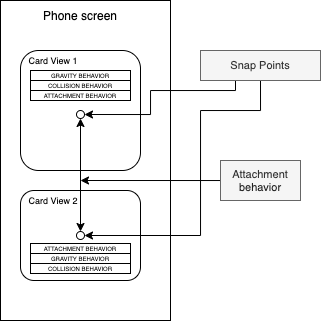
\includegraphics[width=10cm]{animation}
%     \captionof{figure}{
%        Schema dell'implementazione di UIDynamics
%     }
%     \label{fig:6}
% \end{minipage}\\

\section{Scomposizione del requisito}

Per semplicità divido il requisito in diversi punti e per ognuno ne spiego la soluzione
o metodologia utilizzata:

\begin{enumerate}
    \item\label{animationenum:1} Le animazioni devono essere disponibili in qualunque sezione o vista in cui si trovi l'utente e definite dal contesto attuale;

    \item\label{animationenum:2} Ogni CardView deve essere trascinabile dall'utente;
    
    \item\label{animationenum:3} Nel momento in cui l'utente usa una forza di trascinamento superiore a un valore di soglia tutte le viste devono
        cadere per gravità;

    \item\label{animationenum:4} Ogni CardView mostrerà un contenuto dinamico differente e definito da dei componenti
    limitati specifici

    \item\label{animationenum:5} Le animazioni in questione devono essere progettate in pagine, in cui ogni pagina può contenere 
    più CardView. L'utente vedrà in un determinato momento una e soltanto una pagina. 
    Una volta che le CardView acquisisco una gravità e cadono, finirà l'animazione o apparirà
    una nuova pagina, se presente;

    \item\label{animationenum:7} Ogni CardView deve interagire con le altre della stessa pagina, come se si toccassero;

\end{enumerate}

% % % % % % % % % % % % % % % % % % % % % % % % % % % % % % % % % % % % %
%                      Onnipresenza delle animazioni                    %
% % % % % % % % % % % % % % % % % % % % % % % % % % % % % % % % % % % % %
\subsection{~\ref{animationenum:1}. Presentazione delle animazioni}

Per creare animazioni definite dal contesto usiamo quindi un semplice UIViewController che gestirà tutte le animazioni,
ma invece di presentarlo attraverso i metodi base visti alla sezione~\ref{sec:navigation}, lo presentiamo al di sopra della \textbf{UIWindow} (vedere sezione~\ref{sec:uiwindow}),
in modo da non essere vincolati dal contesto dell'utente quando l'animazione finirà, ma allo stesso tempo
consentire il controllo dell'inizializzazione del UIViewController in base al contesto attuale.

\subsection{Aggiunta del ViewController nella\\UIWindow}

L'animazione viene inizializzata nel ViewController, in questo caso \textbf{mainViewController},
genitore di tutto il contesto, in modo da avere il controllo su tutto 
il contesto. Questo perchè tutti i ViewController nello stack di navigazione possono
essere chiusi a seguito di un qualunque eventi dell'animazione, avendo così un controllo molto accuranto
del contenuto che l'utente visualizzerà alla fine dell'animazione.

\begin{minted}{swift}
let keyWindow: UIWindow?

if #available(iOS 13.0, *) {
    keyWindow = UIApplication.shared.connectedScenes
    .filter({$0.activationState == .foregroundActive})
    .map({$0 as? UIWindowScene})
    .compactMap({$0})
    .first?.windows
    .filter({$0.isKeyWindow}).first
} else {
    keyWindow = UIApplication.shared.keyWindow
}

mainViewController.addChild(currentAnimationViewController!)

// Aggiungiamo la vista del nostro viewController alla UIWindow
keyWindow?.addSubview(currentAnimationViewController!.view)

// Rimuoviamo il viewController
currentAnimationViewController!.didMove(toParent: mainViewController)
\end{minted}

% % % % % % % % % % % % % % % % % % % % % % % % % % % % % % % % % % % % %
%                        CardView trascinabile                          %
% % % % % % % % % % % % % % % % % % % % % % % % % % % % % % % % % % % % %
\subsection{~\ref{animationenum:2}. Aggiunta di una gesture}\label{gestureimplemention}

Per un'animazione che ha necessità di muoversi come se l'utente la stesse spostando trascinando sullo schermo occore una \textbf{UIPanGestureRecognizer}.
Dalla doumentazione delle UIGestureRecognizer viene spiegato che ogni vista "draggabile" necessita una  e solo una gesture,
per questo ogni card view dovrà averne una diversa. Di seguito il codice di implementazione

\begin{minted}{swift}
// Durante il settaggio delle cardview
// aggiungo la vista alla parentView
parentView.addSubview(view)

// Creo la gesture
let panGesture = UIPanGestureRecognizer(target: target, action: action)

// Assegno un nome che verrà utilizzato come lock
// per impedire la concorrenza di due gesture differenti
panGesture.name = "gesture-\(index)"

// Aggiungo la gesture alla cardView
cardView.addGestureRecognizer(panGesture)
\end{minted}

I parametri target e action sono rispettivamente il viewController che gestisce la gesture e il metodo
che deve essere eseguito quando avviene una PanGesture.
Di seguito l'implementazione del metodo handlePan che gestisce tutte le gesture di una stessa pagina.

\begin{minted}{swift}
private let activeGesture = nil

// Metodo chiamato dalla UIPanGesture
@objc private func handlePan(_ recognizer: UIPanGestureRecognizer) {
    // Lock per evitare che due gesture funzionino in contemporanea
    if let gestureName = activeGesture, recognizer.name != gestureName {
        return
    } else {
        activeGesture = recognizer.name
    }
    
    // CardView che viene mossa dall'utente
    let animatedView = recognizer.view!
    
    // Coordinate del punto di tocco rispetto alla vista principale
    let touchPointInView = recognizer.location(in: self.view)

    // Coordinate del punto di tocco rispetto alla cardView
    let touchPointInAlert = recognizer.location(in: animatedView)
    let velocity = recognizer.velocity(in: self.view)
    
    // Ottengo l'offset rispetto al centro della cardView
    let offset = UIOffset(
        horizontal: touchPointInAlert.x - animatedView.bounds.midX,
        vertical: touchPointInAlert.y - animatedView.bounds.midY
    )

    // Aggingo i comportamenti iniziali
    self.createPageDynamicBehaviours()
    self.addCheckForDismiss()
    
    // Attivo e disattivo i comportamenti del UIDynamicAnimator
    // in base agli stati delle PanGesture
    switch recognizer.state {
    case .began:
        self.configureForStartDragging(animatedView,
            with: offset,
            touchPointInView: touchPointInView,
            touchPointInAlert: touchPointInAlert
        )
    case .changed:
        // Sposto la cardView attraverso un attachmentBehavior
        dragAttachmentBehavior.anchorPoint = touchPointInView
    case .cancelled, .ended, .failed:
        self.configureForFinishDragging(animatedView,
            with: velocity,
            offset: offset
        )
        // Disattivo il lock
        activeGesture = nil
    default:
        break
    }
}
\end{minted}

% % % % % % % % % % % % % % % % % % % % % % % % % % % % % % % % % % % % %
%                        Gravity                                     %
% % % % % % % % % % % % % % % % % % % % % % % % % % % % % % % % % % % % %
\subsection{~\ref{animationenum:3}. Aggiunta della gravità }

Attraveso la UIPanGesture è possibile calcolare il vettore della velocità del trascinamento,
con questo semplice dato e ciò che abbiamo studiato dello UIKit Dynamics è possibile aggiungere una gravità solo se
il vettore della velocità è superiore a una soglia prestabilita.

Per implementarlo è stato utilizzato un UIGravityBehavior, inizializzato in questo modo:

\begin{minted}{swift}
    let gravityBehavior = UIGravityBehavior(items: page.views)
    gravityBehavior.magnitude = Constants.gravity
\end{minted}

Il valore \textbf{magnitude} è la forza di gravità che vogliamo
assegnare alle viste in questione. \\

Nella figura~\ref{fig:6} si vede lo schermo di uno smartphone, che presenta l'animazione
voluta in questo caso con due CardView. Ognuna di esse ha un \textbf{UIAttachmentBehavior} al
centro per fare in modo che sia sempre centrata in esso (o nel punto di drag dell'utente),
un \textbf{UICollisionBehavior} per permettere che durante il drag le CardView possa scontrarsi e non si accavallino e un \textbf{UIGravityBehavior}, il quale 
viene utilizzato per la caduta delle viste alla fine dell'animazione o al cambiamento di pagina.

In più esiste uno speciale UIAttachmentBehavior tra i centri delle due CardView per permettere che il movimento di una
sposti anche l'altra, è una sorta di corda che le lega.

Per l'ingresso invece è stato inserito un UISnapBehavior, al centro per ogni oggetto, che anima 
gli oggenti dando un effetto a molla.

Tutte le animazione sono attivate e disattive in specifici momenti, questo dipende 
dalla UIPanGestureRecognizer e dai movimenti dell'utente.

% % % % % % % % % % % % % % % % % % % % % % % % % % % % % % % % % % % % %
%                        Modular CardView                               %
% % % % % % % % % % % % % % % % % % % % % % % % % % % % % % % % % % % % %
\subsection{~\ref{animationenum:4}. La CardView modulare}

L'intero UIViewControllor che regola le CardView animate è stato progettato per presentare 
animazioni con contenuti dinamici, per questo sono state progettate delle strutture dati specifiche per consentire la personalizzazione
del contenuto di ogni CardView. 

Inizialmente sono stati definiti i possibili componenti che ogni CardView può adottare:
\begin{itemize}
    \item\textbf{Solo testo}: Il componente include un testo, il suo colore e il colore di sfondo
    \item\textbf{Solo Immagine}: Il componente include un'immagine e il colore di sfondo
    \item\textbf{Row}: Il componente include un'icona e due testi in quest'ordine;
    \item\textbf{Animazione Lottie\cite{lottie}}: Il componente include una semplice UIView in cui viene mostrata un'animazione Lottie
    \item\textbf{Footer}: Il componente include del testo e un'icona sulla destra;
\end{itemize}

Una volta definiti tutti i componenti per ogni CardView questa viene assemblata "incollando" un componente
dopo l'altro attraveso una vista chiamata ModularCardView, di seguito, in figura~\ref{fig:7} il risultato finale ottenuto. \\

\begin{minipage}{\linewidth}
    \centering
    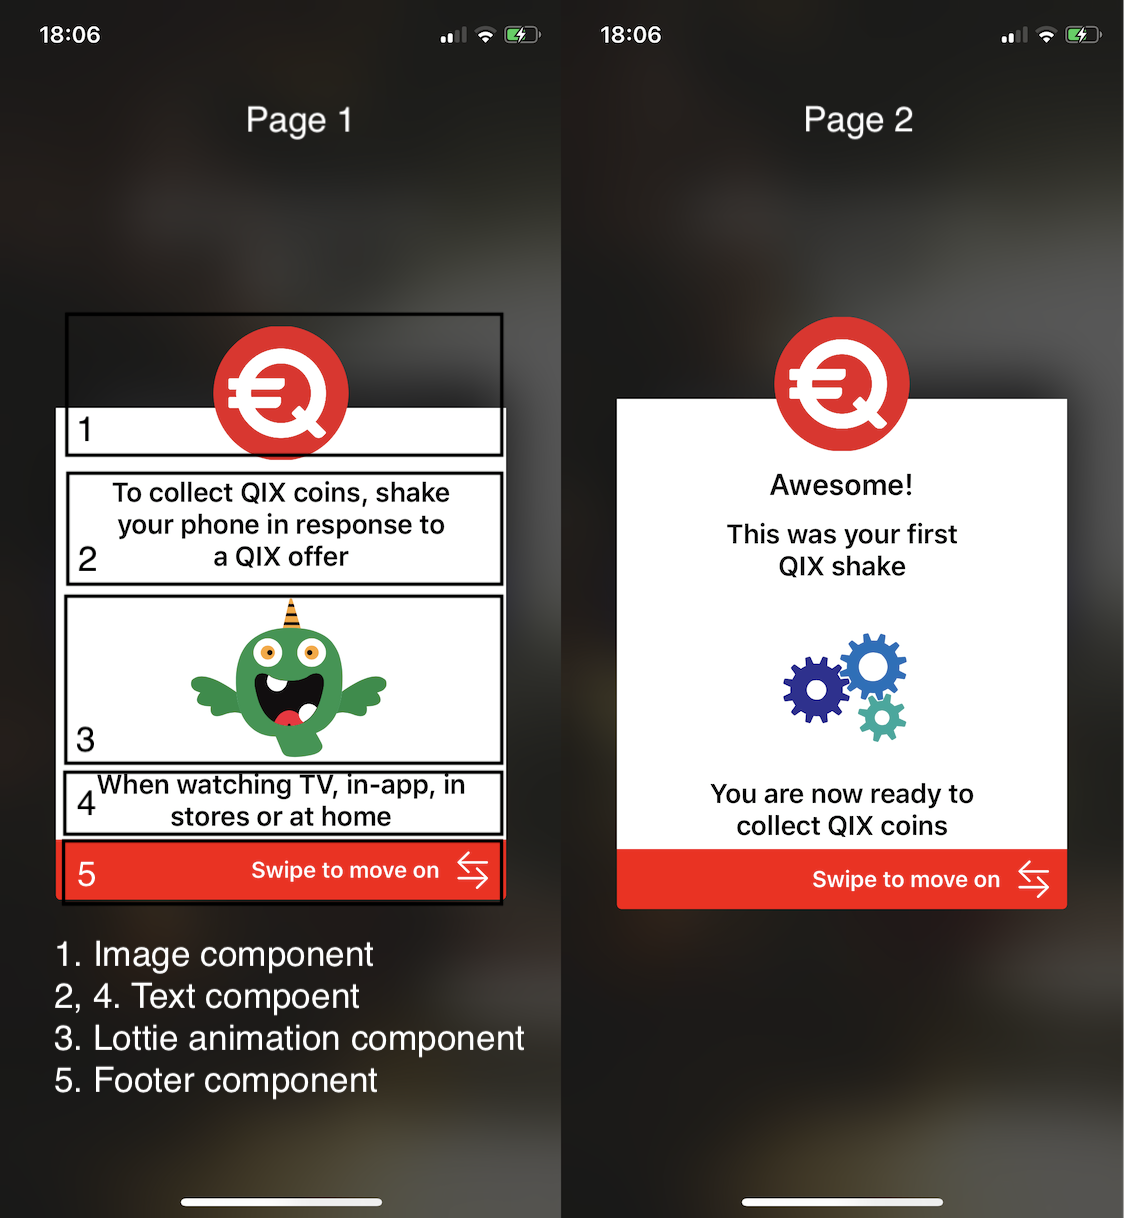
\includegraphics[width=10cm]{an12}
    \captionof{figure}{
       CardViews modulari
    }
    \label{fig:7}
\end{minipage}\\

Dopo aver creato ogni componente separatamente ho creato la \textbf{ModularCardView},
questa vista attraverso un array di UIView, ossia i componenti, utilizza dei constraints 
per assemblarli insieme. Vediamo di seguito il metodo \textbf{build}:

\begin{minted}{swift}
// Creo un array di constraints
var constraints = [NSLayoutConstraint]()
    
// Creo un loop enumerato sull'array dei componenti
for (index, view) in components.enumerated() {
    // Disabilito l'autoresizing mask automatico
    view.translatesAutoresizingMaskIntoConstraints = false
    
    // Aggiugo il componente alla ModulaCardView
    self.addSubview(view)
    
    // Aggiungi i constraint a destra e sinistra
    constraints.append(contentsOf: [
        view.leadingAnchor.constraint(equalTo: self.leadingAnchor),
        view.trailingAnchor.constraint(equalTo: self.trailingAnchor)
    ])
    
    if components.count > 1 {

        if index == 0 {
            // Al primo componente setto il top della ModulaView
            constraints.append(
                view.topAnchor.constraint(equalTo: self.topAnchor)
            )
        } else {
            // Ai sucessivi setto top anchor il bottom
            // anchor dell'elemento precedente
            let bottomAnchor = components[index - 1].bottomAnchor
            constraints.append(
                view.topAnchor.constraint(equalTo: bottomAnchor)
            )
        }
        
        // Se è l'ultimo componente gli aggiugo un constraint
        // alla fine della ModularView
        if index == components.count - 1 {
            constraints.append(
                view.bottomAnchor.constraint(equalTo: self.bottomAnchor)
            )
        }
    } else {
        // Esiste un solo componente,
        // gli setto i constraint sopra e sotto
        constraints.append(contentsOf: [
            view.topAnchor.constraint(equalTo: self.topAnchor),
            view.bottomAnchor.constraint(equalTo: self.bottomAnchor)
        ])
    }
}

// Attivo tutto i constraints
NSLayoutConstraint.activate(constraints)
\end{minted}

% % % % % % % % % % % % % % % % % % % % % % % % % % % % % % % % % % % % %
%                   La paginazione delle animazioni                     %
% % % % % % % % % % % % % % % % % % % % % % % % % % % % % % % % % % % % %
\subsection{~\ref{animationenum:5}. Paginazione delle animazioni}

Avendo definito al punto~\ref{animationenum:1} l'utilizzo di un solo UIViewController per le animazioni da un lato viene semplificata
la presentazione delle stesse, dato che basterà presentare un solo UIViewController, ma dall'altro verrà delegata
l'intera paginagione al view controller. \\

In particolare questo UIViewController accetta come variabile di inizializzazione
un array di pagine e in base allo stato della UIPanGestureRecognir deciderà se passare alla pagina successiva
o interrompere l'animazione;


% % % % % % % % % % % % % % % % % % % % % % % % % % % % % % % % % % % % %
%                   La paginazione delle animazioni                     %
% % % % % % % % % % % % % % % % % % % % % % % % % % % % % % % % % % % % %
\subsection{~\ref{animationenum:5}. Il Collider}

Come accennato al punto~\ref{animationenum:3} ogni le CardView hanno dei comportamenti fisici definiti
da UIkit Dynamics, in particolare per conferire un effetto di collisione viene usato un \textbf{UICollisionBehavior} e implementato come segue:

\begin{minted}{swift}
    let itemsCollisionBehavior = UICollisionBehavior(items: page.views)
\end{minted}

In questo modo ogni ogni oggetto con questo
comportamento riuscirà a scontrasi con gli altri oggetti simili.


    \chapter{Autenticazione}
    \label{CH:6}
    \section{Firebase Authentication}

\section{Tipologie di autenticazione}

Per la progettazionde dell'autenticazione si è voluto ricorrere a qualcosa di 
già pronto per velocizzare i tempi di sviluppo e quindi evitare di progettare e implementare un sistema 
complesso come la gestione di utenti non autenticati (Guest).

Cercando in rete abbiamo optato per l'utilizzo di \textbf{Firebase}\cite{firebase}: ossia una piattaforma
di sviluppo per applicazione mobili e web acquisita di Google nel 2014. 
Uno dei motivi fondamentali per cui è stata scelta è la grande quantità di servizi utili come
analisi dei Crash, tracking della naviazione degli utenti, DynamicLinks (si veda sezione~\ref{section:dynamiclinks})
e ovviamente l'autenticazione.

Esistono 3 tipologie di autenticazione come definito nel requisito, ognuna della quali è un'estensione
di quella precedente: un utente che apre per la prima volta l'applicazione verrà subito registrato 
come utente anonimo e quindi in \textbf{Trial Mdoe}, se poi decide di effettuare la registrazione può inserire 
il suo numero di telefono o la sua email e attraverso Firebase l'utente anonimo evolverà in un utente con più
informazioni, in \textbf{Signed Mode}.

Successivamente ci sarà nell'applicazione una sezione specifica dove l'utente potrà inserire nuovi dati come nome, cognome e data di nascita
o semplicemente potrà linkare un social media come Facebook, Google o Instagram. In questo caso l'utente evolverà nuovamente 
e arriverà nella \textbf{Pro Mode}.

Il pacchetto Firebase Auth infatti include tutte queste funzionalità e attraverso delle semplici API
è possibile utilizzarlo come segue:

Inizializzazione di Firebase nel file di inizializzazione dell'applicazione ossia l'AppDelegate.swift

\begin{minted}{swift}
    FirebaseApp.configure()
\end{minted}

Creazione di un utente anonimo

\begin{minted}{swift}
    Auth.auth().signInAnonymously() { (authResult, error) in
        // ...
    }
\end{minted}

Collegamento di un account anonimo con numero di telefono o email

\begin{minted}{swift}
    // L'oggetto user è sempre disponibile in firebase e
    // salvato nel keychain di iOS
    let user = Auth.auth().currentUser

    // Creazione dell'oggetto credenzial da collegare
    // all'utente attuale (anonimo o non)
    let credential = EmailAuthProvider.credential(withEmail: email,
        password: password)

    // Linking dei due account
    user?.link(with: credential) { (authResult, error) in
        // ...
    }
\end{minted}

Il linking con un qualunque social media è simile all'esempio riportato
qui sopra, cambiare soltanto il Provider delle credenziali

    
    \chapter{Dynamic Links}
    \label{CH:7}
    
Un'altra interessante funzione di Firebase sono i \textbf{Dynamic Links}
ossia dei semplici URL generati dalla console o direttamente dall'applicazione
che consentono la creazione semplificata di particolari \textbf{DeepLink}.

In particolare i DeepLink in Android e iOS sono degli URl che vengono registrati nell'applicazione
e non fanno altro che evitare l'apertura del browser rispetto a quella dell'applicazione.

Questo permette agli utenti di aprire direttamente l'applicazione in questione
attraverso lo smartphone o il computer attraverso il browser, ma trasportando dei dati utili all'azienda.



In particolare ho implementato un sistema di inviti, per cui 
un utente può invitarne un altro attraverso questi link ed è necessario tracciare
l'utente che ha inviato l'invito per inviargli un premio.

Per risolvere il problema abbiamo prima implementato i Dynamic Links attraverso le API de
di Firebase e successivamente nella creazione del link iniettiamo dell'URL un id univoco che identifica l'utente
che crea il link di invito.

\subsection*{Generazione di un DynamicLink}

Attraverso Firebase risulta molto semplice generare il DynamicLink,
l'unica cosa che ci serve è l'id dell'utente

\begin{minted}{swift}
let userId = Configuration.shared.fetchUserId() 

// DeepLink registrato nell'app
let targetLink = URL(string:
    "https://myqix.com/invitation#\(userId)")

// Generato da Firebase
let dynamicLinksDomain = "https://myqix3appdev.page.link"

// Inizializzo la creazione del DynamicLink
let linkBuilder = DynamicLinkComponents(link: targetLink,
    domainURIPrefix: dynamicLinksDomainURIPrefix)

linkBuilder.iOSParameters = 
    DynamicLinkIOSParameters(bundleID: "...")
linkBuilder.iOSParameters?.appStoreID = "1459917691"
linkBuilder.iOSParameters?.minimumAppVersion = "0.0.2"

linkBuilder.androidParameters
    = DynamicLinkAndroidParameters()
linkBuilder.androidParameters?.fallbackURL = link

// Crea un versione del link più piccola
linkBuilder.shorten { url, _, error in
    
    guard let url = url, error == nil else {
        Log.error("Error shorting your URL")
        return
    }
    
    // Completo con l'url generato
    completion(url)
}

\end{minted}

\subsection*{Ottenere i dati}

Ogni volta che un utente clicca su un dynamicLink, iOS controlla
se il link è registrato da qualche app e se questo è il caso
inoltra il link all'app che poi dovrà gestirlo aprendola. 
Il link arriva quindi in una funzione di inizializzazione dell'applicazione all'interno del
file \textbf{AppDelegate}, da cui possiamo analizzare i dati ricevuti e effettuare tutte le operazionni necessarie

\begin{minted}{swift}
// Metodo chiamato allo startup con il dynamic link
func application(_ application: UIApplication,
    continue userActivity: NSUserActivity,
    restorationHandler: 
        @escaping ([UIUserActivityRestoring]?) -> Void) -> Bool {
        
    // Controllo se esiste il link
    if let incomingURL = userActivity.webpageURL {
        // ...
    }
    
    return false
}
\end{minted}
    
    \chapter*{Conclusione}
    \addcontentsline{toc}{chapter}{Conclusione}  
    \label{CH:Concl}
    % Lo sviluppo di QIX è stata una delle esperienze più formative della mia carriera
% studentesca e professionale. Ci sono state molte difficoltà tra cui irequisiti non sempre chiari e
% la complessità dell'applicazione, che mi hanno però sempre spinto a imparare sempre di più e non darmi per viewcontroller.
% Il futuro vede in QIX un'applicazione 
Il mio compito in QIX è stato progettare e implementare, insieme ad un intero team di sviluppo, 
l'applicazione QIX basandosi su dei requisiti base definiti dal team a seguito di molti meeting 
e brain storming. L'applicazione è ancora agli inizi, una prima versione potrebbe già essere.
negli store questo inverno.
    
    \bibliographystyle{unsrt}
    \bibliography{bibliography}
    
    \listoffigures
\end{document}
